\documentclass{exam}
\usepackage{../../mypackages}
\usepackage{../../macros}

\title{DST N°2 - Géométrie dans l'espace et Suites}
\author{N. Bancel}
\date{4 Décembre 2024}

\begin{document}

\textbf{Collège Lycée Suger}
\hfill
\textbf{Mathématiques} \\

\textbf{Année 2024-2025}
\hfill
\textbf{1ères STD2A} \par

{\let\newpage\relax\maketitle}

\begin{center}
\textbf{\textcolor{red}{Durée : 2 heures. La calculatrice n'est pas autorisée}} \\
\textbf{\textcolor{red}{Une réponse donnée sans justification sera considérée comme fausse.}} \\
Cette interrogation contient \numquestions\ questions, sur \numpages\ pages et est notée sur 21 points. 

\end{center}

\section*{Exercice 1 : Jeux de rôles (8 points)}

\textbf{Extrait du BAC 2017 STD2A Nouvelle Calédonie} \par
\vspace{1em}
Dans les jeux de rôles, on utilise différents types de dés en plus du classique dé à six faces afin
d'obtenir des résultats différents. Les polyèdres réguliers, connus aussi sous le nom de "solides de
Platon", permettent d'obtenir des dés équiprobables, chaque face ayant la même probabilité de
sortir à chaque tirage. Par exemple, un dé à huit faces a la forme d'un octaèdre régulier.

\subsection*{Étude de l'octaèdre régulier}

Un octaèdre régulier peut-être obtenu à partir d'un cube en prenant pour sommets de l'octaèdre les centres des faces du cube.
On a représenté ci-dessous, en perspective parallèle, un octaèdre régulier ABCDEF inscrit dans un cube dont l'arête mesure 2 cm.
Le point O est le point d'intersection des diagonales du quadrilatère ABCD

\begin{figure}[H]
  \centering
  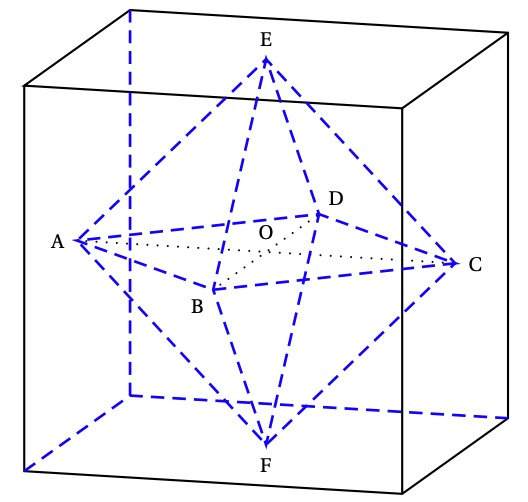
\includegraphics[width=0.4\linewidth]{img/dst_02_01.jpg}
  \caption{\label{} Octaèdre}
\end{figure}

On admet que $\left(O\mathpunct{} ; \ \overrightarrow{OA}\mathpunct{}, \ \overrightarrow{OB}\mathpunct{}, \ \overrightarrow{OE}\right)$ est un repère orthonormal de l'espace.
\begin{questions}
  \question[2.25] \textbf{\textcolor{blue}{Donner les coordonnées des sommets de l'octaèdre régulier ABCDEF dans le repère orthonormal de l'espace $\left(O\mathpunct{} ; \ \overrightarrow{OA}\mathpunct{}, \ \overrightarrow{OB}\mathpunct{}, \ \overrightarrow{OE}\right)$}}

  Le repère étant orthonormal, son unité de "mesure" est 1. $\left(O\mathpunct{} ; \ \overrightarrow{OA}\mathpunct{}, \ \overrightarrow{OB}\mathpunct{}, \ \overrightarrow{OE}\right)$ nous permet de dire que 
  \begin{itemize}
    \item $OA = 1$ La longueur OA vaut 1. Il en est de même pour $OB$ et $OE$. $OA = OB = OE = 1$
    \item En terme de directions : la direction $\overrightarrow{OA}$ indique le sens des "x postifs". La direction $\overrightarrow{OB}$ indique le sens des "y positifs". La direction $\overrightarrow{OE}$ indique le sens des "z positifs".
  \end{itemize}

  Il faut toujours commencer par donner les coordonées des points qui définissent le repère orthonormé. C'est plus simple. Ainsi, on peut donner les coordonées suivantes : 
  \begin{itemize}
    \item $A(1,0,0)$
    \item $B(0,1,0)$
    \item $E(0,0,1)$
    \item C est au même niveau que A sur les Y et les Z, mais il est à l'opposé de A sur les X : $C(-1,0,0)$
    \item D est au même niveau que B sur les X et les Z, mais il est à l'opposé de B sur les Y : $D(0,-1,0)$
    \item F est au même niveau que E sur les X et les Y, mais il est à l'opposé de E sur les Z : $F(0,0,-1)$
  \end{itemize}


  \textbf{Résultat final :} 
\begin{align*}
  A(1; 0; 0) \\
  B(0; 1; 0) \\
  C(-1; 0; 0) \\
  D(0; -1; 0) \\
  E(0; 0; 1) \\
  F(0; 0; -1)
\end{align*} 

  \question[1] \textbf{\textcolor{blue}{Que peut-on dire de la sphère de centre O passant par A ?}}

  On sait que $OA = OB = OE$ par définition du repère orthonormé. Un rapide calcul (et à vue d'oeil en regardant les coordonées), on voit que $OD = OC = OF = 1$. Etant donné que toutes ces longueurs sont égales et que OA correspond au rayon de la sphéère de centre O et de rayon OA, on peut dire que les points OB, OC, OD, OE, OF représentent aussi des rayons et donc que le tétraèdre régulier est exactemnet inclus dans la sphère.

  \question[1] En utilisant les coordonées de $A$ et de $E$, calculer la longueur AE de l'arête de l'octaèdre régulier ABCD.

  Par définition : 

  \[
  AE = \sqrt{(x_A - x_E)^2 + (y_A - y_E)^2 + (z_A - z_E)^2}
  \]

  Donc 

  \begin{align}
    AE &= \sqrt{(1-0)^2 + (0 - 0)^2 + (0 - (-1))^2} \\
    AE &= \sqrt{(1)^2 + (0)^2 + (1)^2} \\
    AE &= \sqrt{2} \\
  \end{align}

  \question[1]\textbf{\textcolor{blue}{Retrouver ce résultat en utilisant le théorème de Pythagore}}

  On sait que le triangle OAE est rectangle en O car le repère $\left(O\mathpunct{} ; \ \overrightarrow{OA}\mathpunct{}, \ \overrightarrow{OB}\mathpunct{}, \ \overrightarrow{OE}\right)$ est orthonomal d'origine O. 
  Donc $(OE)$ est perpendiculaire à $(OA)$, et $OA = OE = 1$. D'après le théorème de Pythagore appliqué au triangle OAE : 

  \begin{align}
  AE^2 &= OE^2 + OA^2 \\
  AE^2 &= 1^2 + 1^2 \\ 
  AE^2 &= 2 \\ 
  AE &= \sqrt{2}
\end{align}

  \question[1] \textbf{\textcolor{blue}{Calculer les coordonées des vecteurs $\overrightarrow{AE}$ et $\overrightarrow{DF}$}}

  \[
  \begin{pmatrix}
    x_{AE} \\
    y_{AE} \\ 
    z_{AE}
  \end{pmatrix}
  = 
  \begin{pmatrix}
    x_{E} - x_{A} \\
    y_{E} - y_{A} \\ 
    z_{E} - z_{A}
  \end{pmatrix}
\]

\[
  \begin{pmatrix}
    x_{AE} \\
    y_{AE} \\ 
    z_{AE}
  \end{pmatrix}
  = 
  \begin{pmatrix}
    0 - 1 \\
    0 - 0 \\ 
    1 - 0
  \end{pmatrix}
  = 
  \begin{pmatrix}
    - 1 \\
    0 \\ 
    1
  \end{pmatrix}
\]

\[
  \begin{pmatrix}
    x_{DF} \\
    y_{DF} \\ 
    z_{DF}
  \end{pmatrix}
  = 
  \begin{pmatrix}
    x_{F} - x_{D} \\
    y_{F} - y_{D} \\ 
    z_{F} - z_{D}
  \end{pmatrix}
\]

\[
  \begin{pmatrix}
    x_{DF} \\
    y_{DF} \\ 
    z_{DF}
  \end{pmatrix}
  = 
  \begin{pmatrix}
    0 - 0 \\
    0 - (-1) \\ 
    -1 - 0
  \end{pmatrix}
  = 
  \begin{pmatrix}
    0 \\
    1 \\ 
    -1
  \end{pmatrix}
\]

  \question[0.75] \textbf{\textcolor{blue}{En utilisant l'annexe et la question précédente, les droites $(AE)$ et $(DF)$ sont-elles perpendiculaires ? Justifier}}

  On calcule le produit scalaire des vecteurs $\overrightarrow{AE}$ et $\overrightarrow{DF}$.

  \[
  \overrightarrow{AE} = 
  \begin{pmatrix}
    x_{AE} \\
    y_{AE} \\ 
    z_{AE}
  \end{pmatrix}
\] et
\[
  \overrightarrow{DF} = 
  \begin{pmatrix}
    x_{DF} \\
    y_{DF} \\ 
    z_{DF}
  \end{pmatrix}
\]
sont orthogonaux si et seulement si leur produit scalaire est égal à 0, c'est-à-dire : 
\[
  x_{AE} \cdot x_{DF} + y_{AE} \cdot y_{DF} + z_{AE} \cdot z_{DF} = 0
\]

\begin{align*}
  \overrightarrow{AE} \cdot \overrightarrow{DF} &= -1 \times 0 + 0 \times 1 + 1 \times -1 \\
  \overrightarrow{AE} \cdot \overrightarrow{DF} &= -1
\end{align*}

Le produit scalaire n'est pas égal à 0, on peut donc en conclure que les 2 droites ne sont pas perpendiculaires.

  \question[1] \textbf{\textcolor{blue}{Calculer le volume de l'octaèdre régulier ABCDEF. On arrondira le résultat au $cm^3$. On rappelle que le volume $V$ d'une pyramide est donné par la formule :
 \[
  V = \frac{B \times h}{3}
  \]
  où $B$ est l'aire de la base de la pyramide et $h$ la hauteur relative à cette base.}}

  La base est un carré ABCD, de côté AB. On sait que l'octaèdre est régulier donc tous ses côtés ont la même longueur. Ainsi, $AB = AE = \sqrt{2}$. La formule de l'aire d'un carré est 
  \[\text{Aire} = \text{côté}^2\]
  Par ailleurs, la hauteur de l'octaèdre est OE, et on sait que OE = 1 (puisque c'est l'unité de mesure sur l'axe Z du répère orthonormé). Donc

  \[
    V = \frac{ AB^2 \times OE }{3}
    \]


  \[
    V = \frac{ \sqrt{2}^2 \times 1 }{3}
    \]

\[
    V = \frac{2}{3} \text{cms}
    \]

\end{questions} 



\section*{Exercice 2 : Le parallélépipède rectangle (8 points)}

On considère le parallélépipède rectangle $ABCDEFGH$ représenté ci-dessous, tel que $AB = 6$, $AD = 4$ et $AE = 2$.

\begin{center}
    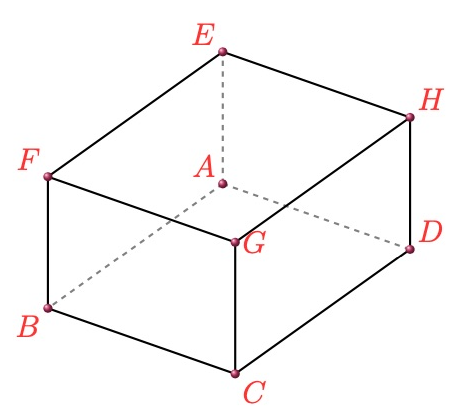
\includegraphics[width=0.5\textwidth]{img/dst_02_02.png}
\end{center}

On se place dans le repère 
\[
\left(A \mathpunct{}; \ \frac{1}{6} \overrightarrow{AB}\mathpunct{}, \ \frac{1}{4} \overrightarrow{AD}\mathpunct{}, \ \frac{1}{2} \overrightarrow{AE}\right).
\]

\begin{questions}
    \question[2] \textbf{\textcolor{blue}{Donner les coordonnées des points $A$, $B$, $C$, $D$, $E$, $F$ et $G$ dans ce repère.}}

    Voici le raisonnement à suivre : $\frac{1}{6} \overrightarrow{AB}\mathpunct{}$ représente le vecteur $\vec{\imath}$, c'est-à-dire l'unité de mesure qui vaut 1. Donc on sait déjà que $AB$ a une longueur de 6. (il vaut 6 fois la distance $\vec{\imath}$). On applique le même raisonnement pour les autres directions du repère. On commence par positionner les trois points clés qui suivent la direction d'un axe précis :

    \[
      \left\{
      \begin{array}{l}
          A(0 ; 0 ; 0) \\
          B(6 ; 0 : 0) \\
          D(0 ; 4 : 0) \\
          E(0 ; 0 : 2) \\
      \end{array}
      \right.
      \]

    Le point "C" prend ce qu'il y a à prendre de D en terme d'avancée sur l'axe des y, et ce qu'il y a à prendre de B sur l'axe des X. Il est au niveau du "sol", donc est à 0 sur l'axe des y. On suit cette même logique pour tous les autres points. Attention à bien prendre des éléments de vérification : F doit avoir le même X que B. H doit avoir le même Y que D. E, F, G, H doivent avoir le même Z etc. 

        \[
      \left\{
      \begin{array}{l}
          C(6 ; 4 ; 0) \\
          F(6 ; 0 : 2) \\
          G(6 ; 4 : 2) \\
          H(0 ; 4 : 2) \\
      \end{array}
      \right.
      \]

    \question[0.5] \textbf{\textcolor{blue}{Donner les coordonnées du vecteur $\overrightarrow{AC}$.}}

    \begin{align*}
      \overrightarrow{AC} &= \begin{pmatrix}
        x_{C} - x_{A} \\
        y_{C} - y_{A} \\ 
        z_{C} - z_{A}
      \end{pmatrix} \\
      \overrightarrow{AC} &= \begin{pmatrix}
        6 - 0 \\
        4 - 0 \\
        0 - 0 \\
      \end{pmatrix} \\
      \overrightarrow{AC} &= \begin{pmatrix}
        6 \\
        4 \\
        0 \\
      \end{pmatrix}
    \end{align*}


    \question[0.5] \textbf{\textcolor{blue}{On considère le point $I$ tel que 
    \[
    \overrightarrow{DI} = \frac{1}{2} \overrightarrow{DH}.
    \]
    Placer le point $I$ sur le graphique. Pas besoin de calcul, vous devez pouvoir placer ce point grâce à la compréhension de la notion de vecteur.}}

    \question[0.5] \textbf{\textcolor{blue}{Donner les coordonnées du point $I$. Bonus : avec une équation (sans utiliser une simple lecture graphique), comment pouvait-on trouver proprement les coordonées du point I ?}}

    Pour déterminer les coordonnées du point $I$, utilisons la relation donnée :

\[
\overrightarrow{DI} = \frac{1}{2} \overrightarrow{DH}.
\]

Calculons tout d'abord le vecteur $\overrightarrow{DH}$ :

\[
\overrightarrow{DH} = 
\begin{pmatrix}
x_H - x_D \\
y_H - y_D \\
z_H - z_D
\end{pmatrix}
=
\begin{pmatrix}
0 - 0 \\
4 - 4 \\
2 - 0
\end{pmatrix}
=
\begin{pmatrix}
0 \\
0 \\
2
\end{pmatrix}.
\]

Ensuite, nous avons :

\[
\frac{1}{2} \overrightarrow{DH} =
\frac{1}{2} \begin{pmatrix}
0 \\
0 \\
2
\end{pmatrix}
=
\begin{pmatrix}
0 \\
0 \\
1
\end{pmatrix}.
\]

En utilisant la définition de $\overrightarrow{DI}$ :

\[
\overrightarrow{DI} = 
\begin{pmatrix}
x_I - x_D \\
y_I - y_D \\
z_I - z_D
\end{pmatrix}
=
\begin{pmatrix}
x_I - 0 \\
y_I - 4 \\
z_I - 0
\end{pmatrix}.
\]

Nous obtenons donc les équations suivantes :

\[
\begin{pmatrix}
x_I - 0 \\
y_I - 4 \\
z_I - 0
\end{pmatrix}
=
\begin{pmatrix}
0 \\
0 \\
1
\end{pmatrix}.
\]

Ce qui donne :

\[
\left\{
\begin{array}{l}
x_I = 0, \\
y_I - 4 = 0 \implies y_I = 4, \\
z_I - 0 = 1 \implies z_I = 1.
\end{array}
\right.
\]

Ainsi, les coordonnées du point $I$ sont :

\[
I(0 ; 4 ; 1).
\]
    


    \question[0.5] \textbf{\textcolor{blue}{En déduire les coordonnées du vecteur $\overrightarrow{EI}$.}}

    Pour déterminer les coordonnées du vecteur $\overrightarrow{EI}$, utilisons la définition :

\[
\overrightarrow{EI} = 
\begin{pmatrix}
x_I - x_E \\
y_I - y_E \\
z_I - z_E
\end{pmatrix}.
\]

Avec les coordonnées de $E(0 ; 0 ; 2)$ et de $I(0 ; 4 ; 1)$, nous avons :

\[
\overrightarrow{EI} = 
\begin{pmatrix}
0 - 0 \\
4 - 0 \\
1 - 2
\end{pmatrix}
=
\begin{pmatrix}
0 \\
4 \\
-1
\end{pmatrix}.
\]

Ainsi, les coordonnées du vecteur $\overrightarrow{EI}$ sont :

\[
\overrightarrow{EI} = 
\begin{pmatrix}
0 \\
4 \\
-1
\end{pmatrix}.
\]

    \question[0.5] \textbf{\textcolor{blue}{Soit $J$ le point défini par 
    \[
    \overrightarrow{FJ} = \overrightarrow{FG} + \frac{1}{2} \overrightarrow{GC}.
    \]
    Placer le point $J$ sur le graphique. Pas besoin de calcul, vous devez pouvoir placer ce point grâce à la compréhension de la notion de vecteur.}}

    \question[0.5] \textbf{\textcolor{blue}{Donner les coordonnées du point $J$. Bonus : avec une équation (sans utiliser une simple lecture graphique), comment pouvait-on trouver proprement les coordonées du point J ?}} 

    Par lecture graphique, on voit que 
    
    \[
    J(6 ; 4; 1)
    \]

    Graphiquement, on voit que J est le milieu de $[GC]$, on peut vérifier en utilisant la formule des coordonées du milieu d'un segment : 

    \begin{align*}
     J &= \begin{pmatrix}
        \frac{x_{C} + x_{G}}{2} \\
        \frac{y_{C} + y_{G}}{2} \\ 
        \frac{z_{C} + z_{G}}{2}
      \end{pmatrix} \\
      J &= \begin{pmatrix}
        \frac{6 + 6}{2} \\
        \frac{4 + 4}{2} \\ 
        \frac{0 + 2}{2}
      \end{pmatrix} \\
      J &= \begin{pmatrix}
        6 \\
        4 \\ 
        1
      \end{pmatrix}
    \end{align*}

    Ceci n'est pas vraiment un raisonnement : le vrai raisonnement correct consiste à résoudre l'équation suivante : 

    \begin{align*}
    \overrightarrow{FJ} &=  \begin{pmatrix}
      x_{J} - x_{F} \\
      y_{J} - y_{F} \\ 
      z_{J} - z_{F} \\
    \end{pmatrix} = \begin{pmatrix}
      x_{J} - 6 \\
      y_{J} - 0 \\ 
      z_{J} - 2 \\
    \end{pmatrix}
  \end{align*}

  \begin{align*}
    \overrightarrow{FG} + \frac{1}{2} \overrightarrow{GC} &=  \begin{pmatrix}
      (x_{G} - x_{F}) + \frac{1}{2} (x_{C} - x_{G}) \\
      (y_{G} - y_{F}) + \frac{1}{2} (y_{C} - y_{G}) \\ 
      (z_{G} - z_{F}) + \frac{1}{2} (z_{C} - z_{G}) \\
    \end{pmatrix} 
  \end{align*}

    \[
\overrightarrow{FG} = 
\begin{pmatrix}
x_G - x_F \\
y_G - y_F \\
z_G - z_F
\end{pmatrix}
=
\begin{pmatrix}
6 - 6 \\
4 - 0 \\
2 - 2
\end{pmatrix}
=
\begin{pmatrix}
0 \\
4 \\
0
\end{pmatrix}
\]


\[
\overrightarrow{GC} = 
\begin{pmatrix}
x_C - x_G \\
y_C - y_G \\
z_C - z_G
\end{pmatrix}
=
\begin{pmatrix}
6 - 6 \\
4 - 4 \\
0 - 2
\end{pmatrix}
=
\begin{pmatrix}
0 \\
0 \\
-2
\end{pmatrix}
\]

\[
\frac{1}{2} \overrightarrow{GC} = 
\frac{1}{2} \begin{pmatrix}
0 \\
0 \\
-2
\end{pmatrix}
=
\begin{pmatrix}
0 \\
0 \\
-1
\end{pmatrix}
\]

Ajoutons ces deux vecteurs :

\[
\overrightarrow{FJ} = 
\overrightarrow{FG} + \frac{1}{2} \overrightarrow{GC} =
\begin{pmatrix}
0 \\
4 \\
0
\end{pmatrix}
+
\begin{pmatrix}
0 \\
0 \\
-1
\end{pmatrix}
=
\begin{pmatrix}
0 \\
4 \\
-1
\end{pmatrix}
\]


En utilisant la définition de $\overrightarrow{FJ}$ :

\[
\overrightarrow{FJ} = 
\begin{pmatrix}
x_J - x_F \\
y_J - y_F \\
z_J - z_F
\end{pmatrix}
=
\begin{pmatrix}
x_J - 6 \\
y_J - 0 \\
z_J - 2
\end{pmatrix}
\]

Nous avons donc :

\[
\begin{pmatrix}
x_J - 6 \\
y_J \\
z_J - 2
\end{pmatrix}
=
\begin{pmatrix}
0 \\
4 \\
-1
\end{pmatrix}
\]

Ce qui donne les équations suivantes :

\[
\left\{
\begin{array}{l}
x_J - 6 = 0 \implies x_J = 6 \\
y_J = 4 \\
z_J - 2 = -1 \implies z_J = 1
\end{array}
\right.
\]

Ainsi, les coordonnées de $J$ sont bien :

\[
J(6 ; 4 ; 1)
\]

    \question[0.5] \textbf{\textcolor{blue}{En déduire les coordonnées du vecteur $\overrightarrow{FJ}$.}}

    Pour déterminer les coordonnées du vecteur $\overrightarrow{FJ}$, utilisons la définition :

    \[
    \overrightarrow{FJ} = 
    \begin{pmatrix}
    x_J - x_F \\
    y_J - y_F \\
    z_J - z_F
    \end{pmatrix}.
    \]
    
    En remplaçant par les coordonnées de $F(6 ; 0 ; 2)$ et de $J(6 ; 4 ; 1)$, on obtient :
    
    \[
    \overrightarrow{FJ} = 
    \begin{pmatrix}
    6 - 6 \\
    4 - 0 \\
    1 - 2
    \end{pmatrix}
    =
    \begin{pmatrix}
    0 \\
    4 \\
    -1
    \end{pmatrix}.
    \]
    
    Ainsi, les coordonnées du vecteur $\overrightarrow{FJ}$ sont :
    
    \[
    \overrightarrow{FJ} = \begin{pmatrix}
    0 \\
    4 \\
    -1
    \end{pmatrix}.
    \]

    \question[1] \textbf{\textcolor{blue}{Quelle est la nature du quadrilatère $EIFJ$ ? Justifier. (On peut utiliser l'information en annexe pour s'aider à répondre à cette question)}}

    D'après les questions précédentes : 

    \[
      \overrightarrow{EI} = \overrightarrow{FJ} = \begin{pmatrix}
        6 \\
        -4 \\
        1
        \end{pmatrix}
  \]

    Les deux vecteurs sont égaux, ils sont donc 
    \begin{itemize}
      \item Colinéaires (donc les droites (EI) et (JF) sont parallèles
      \item De même longueur (donc EI = JF)
    \end{itemize}

    On peut donc en conclure que le quadrilatère EIJF est un parallélogramme. 

    On sait que ABCDEFGH est un parallélépipède rectangle donc les plans (ABFE) et (FGCB) sont orthogonaux. (EF) appartient au lan (ABFE) et (FJ) appartient au plan (FGCB) donc (EF) et (FJ) sont perpendiculaires. 
    On peut donc en déduire que EIJF est un rectangle.

    \question[1] \textbf{\textcolor{blue}{Calculer la longueur des segments $[EF]$ et $[EI]$.}}

    Pour calculer la longueur des segments $[EF]$ et $[EI]$, utilisons la formule de la distance entre deux points dans l'espace :

\[
d(A, B) = \sqrt{(x_B - x_A)^2 + (y_B - y_A)^2 + (z_B - z_A)^2}.
\]

\textbf{1. Longueur du segment $[EF]$ :}

Les coordonnées de $E$ et $F$ sont respectivement $E(0 ; 0 ; 2)$ et $F(6 ; 0 ; 2)$. Ainsi, nous avons :

\[
[EF] = \sqrt{(x_F - x_E)^2 + (y_F - y_E)^2 + (z_F - z_E)^2}.
\]

Substituons les valeurs :

\[
[EF] = \sqrt{(6 - 0)^2 + (0 - 0)^2 + (2 - 2)^2}.
\]

\[
[EF] = \sqrt{6^2 + 0^2 + 0^2} = \sqrt{36} = 6.
\]

\textbf{2. Longueur du segment $[EI]$ :}

Les coordonnées de $E$ et $I$ sont respectivement $E(0 ; 0 ; 2)$ et $I(0 ; 4 ; 1)$. Ainsi, nous avons :

\[
[EI] = \sqrt{(x_I - x_E)^2 + (y_I - y_E)^2 + (z_I - z_E)^2}.
\]

Substituons les valeurs :

\[
[EI] = \sqrt{(0 - 0)^2 + (4 - 0)^2 + (1 - 2)^2}.
\]

\[
[EI] = \sqrt{0^2 + 4^2 + (-1)^2} = \sqrt{0 + 16 + 1} = \sqrt{17}.
\]

\textbf{3. Résultats :}

\[
\text{Longueur de } [EF] = 6, \quad \text{Longueur de } [EI] = \sqrt{17}.
\]

    \question[0.5] \textbf{\textcolor{blue}{En déduire l'aire du quadrilatère $EIFJ$.}}

    Puisque le quadrilatère $EIFJ$ est un rectangle, son aire peut être calculée en utilisant la formule de l'aire d'un rectangle, qui est le produit des longueurs de deux côtés adjacents.
    \[
[EF] = 6.
\]
\[
[EI] = \sqrt{17}
\]
L'aire du rectangle $EIFJ$ est donc le produit de ces deux longueurs :

\[
\text{Aire de } EIFJ = [EF] \times [EI] = 6 \times \sqrt{17}.
\]

\[
\boxed{6\sqrt{17}}.
\]

\end{questions}

\section*{Exercice 3 : Suites - Exercice identique à celui du BAC Blanc. (5 points)}

\begin{questions}
  \question[2.5] Soit $(U_n)$ définie par :
  \[
    \left\{
      \begin{array}{ll}
        U_{n+1} = U_n + n \\
        U_0 = 2
      \end{array}
    \right.
  \]

  \begin{parts}
    \part[1] \textbf{Calcul des quatre premiers termes :} \\
    \textcolor{red}{Attention : dans cette partie, 2 notions sont mixées : la notion d'indice ($n$) et de terme ($U_n$). A chaque calcul d'un nouveau terme : le terme précédent $U_n$ ainsi que l'indice lui même $n$ entrent en jeu}
    \[
    U_0 = 2.
    \]
    Pour $n = 0$ :
    \[
    U_1 = U_0 + 0 = 2 + 0 = 2.
    \]
    Pour $n = 1$ :
    \[
    U_2 = U_1 + 1 = 2 + 1 = 3.
    \]
    Pour $n = 2$ :
    \[
    U_3 = U_2 + 2 = 3 + 2 = 5.
    \]
    Donc, les quatre premiers termes sont : $U_0 = 2$, $U_1 = 2$, $U_2 = 3$, $U_3 = 5$. \\
    Que l'on peut aussi écrire : $\left\{2, 2, 3, 5, ...\right\}$

    \part[1] \textbf{Calcul de $U_{n+1} - U_n$ :}
    Par définition 
    \[
    U_{n+1} = U_n + n
    \]
    donc 
    \[
   \begin{aligned}
    U_{n+1} - U_n &= (U_n + n) - U_n \\
                 &= n.
   \end{aligned} 
   \] \\ 

   \textcolor{red}{Cela pouvait se vérifier rapidement avec quelques exemples : }

   Pour $n = 0$
   \[
    \begin{aligned}
    U_{n+1} - U_n &= U_1 - U_0 \\
      \text{or} \quad U_1 = 2 \quad \text{et} & \quad U_0 = 2 \\ 
      \text{donc} \quad U_{n+1} - U_n &= 2 - 2 \\
                  &= 0
  \end{aligned} 
  \]
  Ce qui correspond bien à la valeur de $n$ ($n=0$)

  Pour $n = 1$
  \[
   \begin{aligned}
   U_{n+1} - U_n &= U_2 - U_1 \\
     \text{or} \quad U_1 = 3 \quad \text{et} & \quad U_1 = 2 \\ 
     \text{donc} \quad U_{n+1} - U_n &= 3 - 2 \\
                 &= 1
 \end{aligned} 
 \]
 Ce qui correspond bien à la valeur de $n$ ($n=1$)


    \part[0.5] \textbf{La suite est-elle croissante ou décroissante ?} \\
    D'après la question précédente, $U_{n+1} - U_n = n$ \\ 
    Or on sait que n est toujours positif : $n \geq 0$.
    
    \[
      \begin{aligned}
      U_{n+1} - U_n &= n \\
        \text{or} \quad n &\geq 0 \\
        \text{donc} \quad U_{n+1} - U_n &= n \geq 0 \\
        U_{n+1} - U_n & \geq 0
    \end{aligned} 
    \]
    
    La suite $(U_n)$ est donc \textbf{strictement croissante}.
  \end{parts}

  \question[3] Soit $(V_n)$ définie par :
  \[
  V_n = 5 \times 2^n.
  \]

  \begin{parts}
    \part[1] \textbf{Calcul des termes $V_0$, $V_1$, et $V_2$ :}
    \[
    V_0 = 5 \times 2^0 = 5 \times 1 = 5.
    \]
    \[
    V_1 = 5 \times 2^1 = 5 \times 2 = 10.
    \]
    \[
    V_2 = 5 \times 2^2 = 5 \times 4 = 20.
    \]
    Donc, $V_0 = 5$, $V_1 = 10$, $V_2 = 20$.

    \part[1] \textbf{Calcul du rapport $\frac{V_{n+1}}{V_n}$ :}
    \[
    \frac{V_{n+1}}{V_n} = \frac{5 \times 2^{n+1}}{5 \times 2^n} 
    = \frac{2^{n+1}}{2^n}
    = \frac{2^n \times 2}{2^n}
    = 2.
    \]

    \part[0.5] \textbf{La suite est-elle géométrique ? Si oui, quelle est sa raison ?} \\
    Oui, $(V_n)$ est une suite géométrique, car $\frac{V_{n+1}}{V_n}$ est constant et vaut $2$. La raison est $q = 2$. \\
    D'après le cours, la suite $(V_n)$ est \textbf{strictement croissante}, car $q > 1$ et $V_n > 0$.
  \end{parts}
\end{questions}

\section*{Partie 3 : Suites arithmétiques et géométriques (3 points)}

\begin{questions}
  \question[1.5] Soit $(W_n)$ définie par :
  \[
    \left\{
      \begin{array}{ll}
        W_{n+1} = W_n + 4 \\
        W_1 = 6
      \end{array}
    \right.
  \]

  \begin{parts}
    \part[0.5] \textbf{La suite est-elle arithmétique ou géométrique ?}
    La suite $(W_n)$ est \textbf{arithmétique} avec une raison $r = 4$, car elle est définie sous la forme 
    
    \[
    W_{n+1} = W_n + r
    \]

    où $r$ est une constante ($r$ vaut 4)

    \part[1] \textbf{Calcul de $W_4$ et $W_6$ :}
    Pour calculer $W_4$, nous procédons en calculant chaque terme de la suite jusqu'à $W_4$ :

\[
W_1 = 6 \quad \text{(donné dans l'énoncé)}.
\]
\[
W_2 = W_1 + 4 = 6 + 4 = 10.
\]
\[
W_3 = W_2 + 4 = 10 + 4 = 14.
\]
\[
W_4 = W_3 + 4 = 14 + 4 = 18.
\]

Ainsi, \( W_4 = 18 \).

---

Pour calculer $W_6$, nous continuons à partir des termes précédents jusqu'à $W_6$ :

\[
W_5 = W_4 + 4 = 18 + 4 = 22.
\]
\[
W_6 = W_5 + 4 = 22 + 4 = 26.
\]

Ainsi, \( W_6 = 26 \).

\textbf{Conclusion :} En calculant chaque terme successivement, nous obtenons :
\[
W_4 = 18 \quad \text{et} \quad W_6 = 26.
\]
  \end{parts}

\end{questions}
\end{document}
